\documentclass[12pt]{article}

\usepackage{sbc-template}
\usepackage[brazil,american]{babel}
\usepackage[utf8]{inputenc}

\usepackage{graphicx}
\usepackage{url}
\usepackage{float}
\usepackage{listings}
\usepackage{color}
\setlength{\marginparwidth}{2cm}
\usepackage{todonotes}
\usepackage{algorithmic}
\usepackage{algorithm}
\usepackage{hyperref}
\usepackage{plantuml}

\sloppy


\title{Trabalho Prático\\ 
Cartolitos CF}

%author{Nome do Aluno, Matrícula\\
\author{Élvis Júnior, 24/1038700\\
        Gustavo Alves, 24/1020779\\
        Pedro Marcinoni, 24/1002396\\
        Grupo 1
}

\address{Dep. Ciência da Computação -- Universidade de Brasília (UnB)\\
  CIC0197 - Técnicas de Programação I\\
  \email{elvismirandajr@gmailcom, gusfring.a@gmail.com, pedroextrer@gmail.com}
}

\begin{document}
\maketitle

\selectlanguage{american}
\begin{abstract}
  This document describes the final project of the course "Técnicas de Programação I" at Universidade de Brasília. The project is a desktop application that allows users to manage their fantasy football teams, providing features such as team creation, player selection, and match simulation. The application is built following object-oriented programming principles and utilizes design patterns to ensure maintainability and scalability.
\end{abstract}
\selectlanguage{brazil}

\begin{resumo}
  Este documento descreve o projeto final da disciplina Técnicas de Programação I da Universidade de Brasília. O projeto é uma aplicação desktop que permite aos usuários gerenciar suas equipes de futebol \textit{fantasy}, oferecendo recursos como criação de equipes, seleção de jogadores e simulação de partidas. A aplicação é construída seguindo princípios de programação orientada a objetos e utiliza padrões de design para garantir manutenibilidade e escalabilidade.
\end{resumo}


\section{Descrição do Problema}
\label{sec:descricao}

Como bons brasileiros, quem não gosta de futebol? Foi pensando nisso que a emissora mais famosa do país, a Rede Globe, criou a Cartolitos CF, o novo Fantasy Game do momento, que reflete em tempo real os resultados estatísticos da Copa do Mundo de Clubes, o mais novo fenômeno do futebol. Veja também \cite{wiki:cartola,wiki:fantasy}.

Disponível para computador, o aplicativo permite que os usuários escalem seus times comprando jogadores dos 32 clubes do torneio com “cartoletas” — a moeda virtual do jogo — e pontue de acordo com o desempenho real desses atletas em campo na rodada. Assim, os participantes podem comparar seus resultados com os amigos em uma liga estilo tiro-curto, na qual se considera apenas uma única rodada.

Para colocar esse projeto em prática, a empresa designou três estudantes de Ciência da Computação — Elvis Miranda, Gustavo Alves e Pedro Marcinoni — para desenvolver um programa capaz de auxiliar na logística de gestão de qualquer liga de tiro-curto, servindo depois como base para o funcionamento integral do aplicativo.

\begin{figure}[H]
  \centering
  \includegraphics[width=0.4\textwidth]{LogoCartolitos.png}
  \caption{Cartolitos CF - Fantasy Game}
  \label{fig:cartolitos}
\end{figure}


\section{Definição das regras de negócio e divisão das tarefas}
\label{sec:regras}

\subsection{Regras de negócio}

\begin{enumerate}
  \item Função do programa:
        \begin{enumerate}
          \item Cadastrar usuários, clubes, jogadores e equipes de usuários
          \item Simula estatísticas e pontuações conforme regras de negócios
          \item era resultados da liga e rankings
        \end{enumerate}
  \item Identificação: Cada usuário tem ID único, nome, e-mail e senha.
  \item Orçamento: Cada usuário começa com 150 cartoletas.
  \item Escalação:
        \begin{enumerate}
          \item O time do usuário deve ter formação 4-3-3, ou seja, 1 goleiro, 4 defensores, 3 meio-campistas e 3 atacantes.
          \item O time do usuário não pode ter jogadores duplicados.
        \end{enumerate}
  \item Capitão: Cada time deve ter um capitão, que recebe o dobro de pontos.
  \item Estatísticas dos jogadores:
        \begin{enumerate}
          \item Cada jogador possui um preço base e uma nota (overall) que varia de 0 a 100.
          \item Cada confronto (casa/fora) usa as notas de cada jogador para ajustar as probabilidades de contribuir com gols, assistências, desarmes, etc.
        \end{enumerate}
  \item Pontuação:
        \begin{enumerate}
          \item Goleiros:
                \begin{itemize}
                  \item Defesa de pênalti: +7 pontos
                  \item Defesa: +1.5 pontos
                  \item Gol sofrido: -1 ponto
                  \item Não sofrer gol: +5 pontos
                \end{itemize}
          \item Defensores:
                \begin{itemize}
                  \item Desarme: +1.5 pontos
                  \item Falta cometida: -0.5 pontos
                  \item Gol contra: -5 pontos
                  \item Cartão amarelo: -1 pontos
                  \item Cartão vermelho: -3 pontos
                \end{itemize}
          \item Meio-campistas:
                \begin{itemize}
                  \item Assistência: +5 pontos
                  \item Gol: +8 pontos
                  \item Falta cometida: -0.5 pontos
                  \item Desarme: +1.5 pontos
                \end{itemize}
          \item Atacantes:
                \begin{itemize}
                  \item Gol: +8 pontos
                  \item Assistência: +5 pontos
                  \item Finalização: +0.8 pontos
                  \item Falta cometida: -0.5 pontos
                \end{itemize}
        \end{enumerate}
  \item Simulação de partidas: O administrador do programa pode simular partidas entre os times cadastrados, gerando estatísticas e pontuações para cada jogador.
  \item Resultados da liga: O programa deve gerar resultados da liga, mostrando a pontuação total de cada time e o ranking dos usuários.
\end{enumerate}

\subsection{Divisão das Tarefas entre os Integrantes}
\label{sec:divisao_tarefas}

A seguir está a divisão das tarefas realizada para o desenvolvimento do projeto final, buscando manter o equilíbrio entre as responsabilidades e funcionalidades implementadas por cada integrante:

\begin{itemize}
  \item \textbf{Élvis Miranda}
        \begin{itemize}
          \item Telas: Login/Cadastro de Usuário, Visualização de Jogadores, Edição de Perfil, Menu Principal do Usuário
          \item Classes: Usuário, Jogador, Posição, Stats, autenticação
          \item Funcionalidades: Cadastro, login, edição de perfil, consulta de jogadores, autenticação
          \item Relatório: Descrição das telas de login, cadastro, visualização de jogadores e perfil; documentação das classes relacionadas
        \end{itemize}
  \item \textbf{Pedro Marcinoni}
        \begin{itemize}
          \item Telas: Montagem do Time, Clubes, Mercado, Edição de Clubes, Menu Principal do Administrador
          \item Classes: TimeUsuario, Clube, manipulação de jogadores no time
          \item Funcionalidades: Montagem e escalação do time, gerenciamento de clubes, mercado de jogadores
          \item Relatório: Descrição das telas de montagem, clubes e mercado; documentação das classes relacionadas
        \end{itemize}
  \item \textbf{Gustavo Alves}
        \begin{itemize}
          \item Telas: Simulação de Partidas, Ranking da Liga, Gerenciamento de Ligas, Gerenciamento de Usuários, Gerenciamento de Partidas
          \item Classes: Partida, Liga, Simulação, pontuação dos times
          \item Funcionalidades: Simulação de partidas, geração de ranking, gerenciamento de ligas, usuários e partidas
          \item Relatório: Descrição das telas de simulação, ranking, gerenciamento de ligas, usuários e partidas; documentação das classes relacionadas
        \end{itemize}
\end{itemize}

Essa divisão permitiu que todos os integrantes participassem ativamente de diferentes etapas do desenvolvimento, garantindo uma contribuição equilibrada e colaborativa para o sucesso do projeto. Apesar de cada integrante ter focado em áreas específicas, todos colaboraram na integração das funcionalidades e na revisão do código, assegurando a coesão do sistema como um todo.

\section{Diagrama de classes final}
\label{sec:classes}

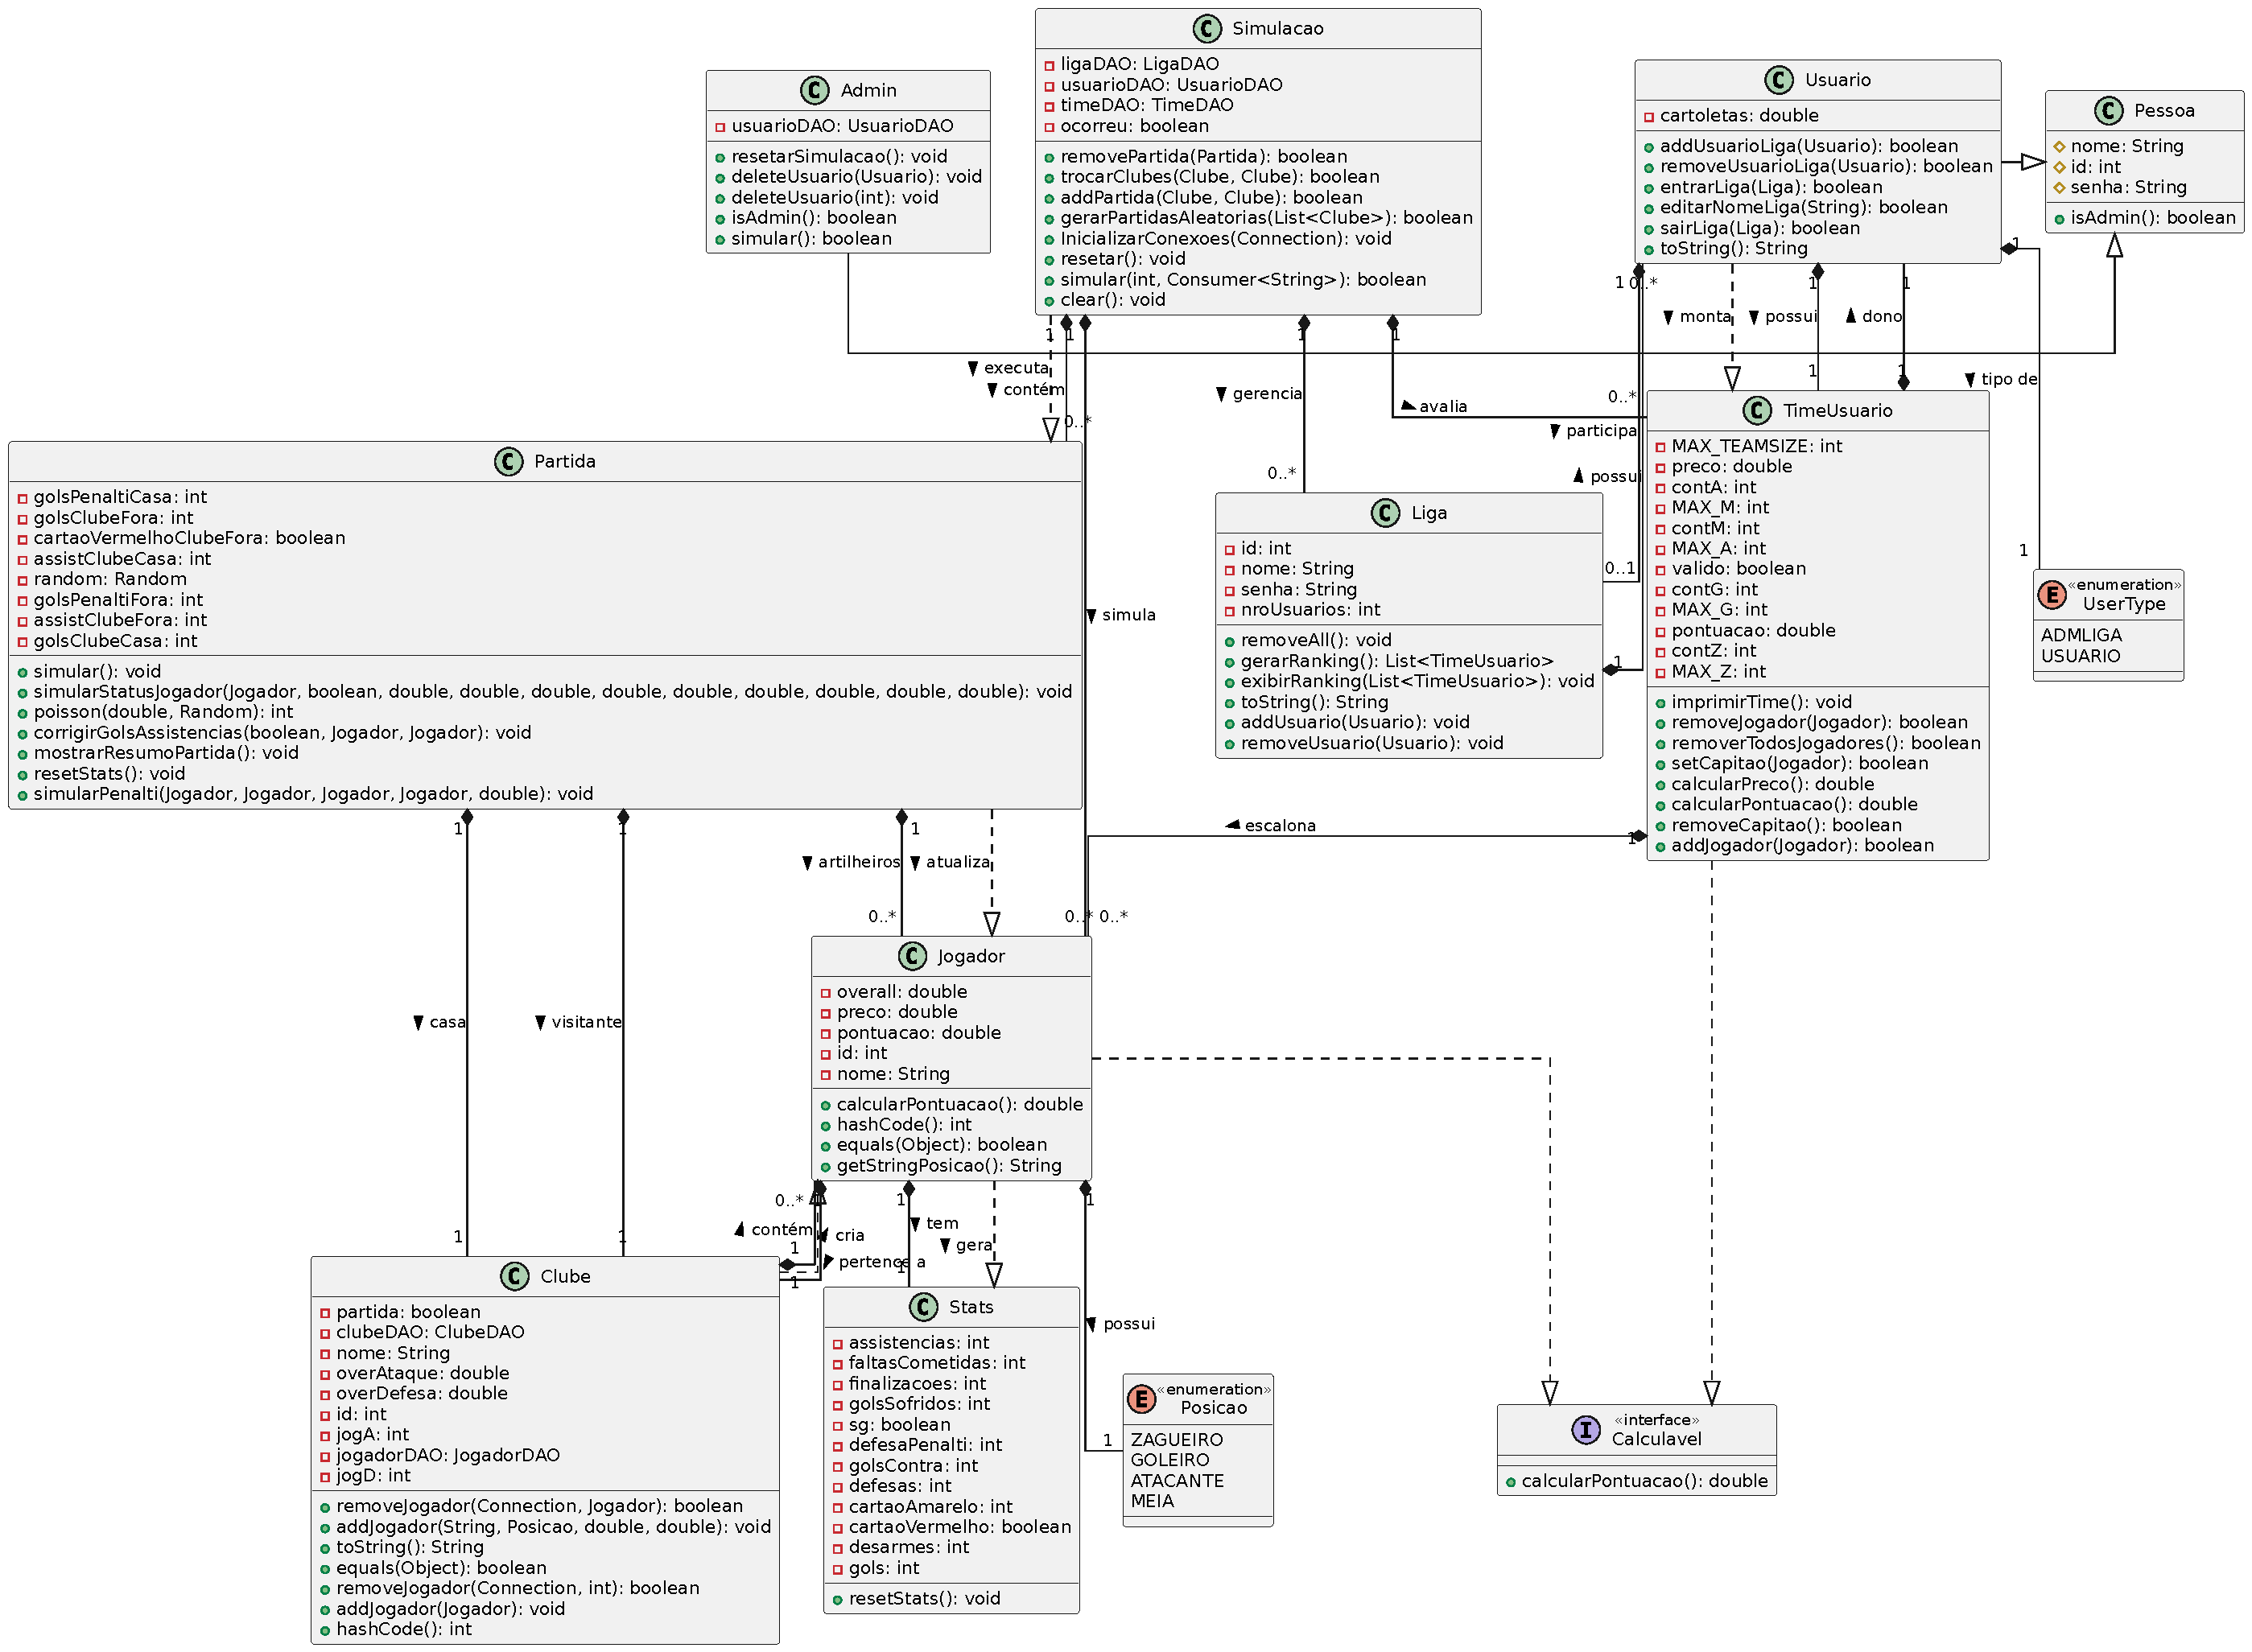
\includegraphics[width=\textwidth]{Diagrama.pdf}

\subsection{Classe abstrata Pessoa}

A classe \textbf{Pessoa} é uma classe abstrata que representa uma pessoa genérica no sistema. Ela possui os seguintes \textbf{atributos}:

\begin{itemize}
  \item \texttt{id}: um identificador único para cada pessoa.
  \item \texttt{nome}: armazena o nome da pessoa.
  \item \texttt{senha}: armazena a senha da pessoa para autenticação.
\end{itemize}

Além disso, a classe define os seguintes \textbf{métodos} (excluindo getters e setters):

\begin{itemize}
  \item \textbf{Construtor \texttt{Pessoa(int id, String nome, String senha)}}: inicializa os atributos \texttt{id}, \texttt{nome} e \texttt{senha} ao criar uma nova instância da classe (ou de suas subclasses).
  \item \textbf{\texttt{isAdmin()}}: método que retorna \texttt{false} por padrão, indicando que a pessoa não é administradora. Esse método pode ser sobrescrito em subclasses para indicar se uma pessoa é administradora do sistema.
\end{itemize}

A classe serve como base para outras classes que representam tipos específicos de pessoas, permitindo reutilização e especialização de comportamento.

\subsubsection{Sublasse Usuario}

A classe \textbf{Usuario} é uma subclasse de \texttt{Pessoa} que representa um usuário do sistema, com funcionalidades específicas para participação em ligas e gerenciamento de seu time. Os principais \textbf{atributos} são:

\begin{itemize}
  \item \texttt{cartoletas}: saldo virtual do usuário, utilizado para comprar jogadores (inicialmente 150).
  \item \texttt{tipo}: indica o tipo do usuário, podendo ser comum ou administrador de liga.
  \item \texttt{timeUsuario}: referência ao time montado pelo usuário.
  \item \texttt{liga}: referência à liga da qual o usuário faz parte.
\end{itemize}

Os principais \textbf{métodos} (excluindo getters e setters) são:

\begin{itemize}
  \item \texttt{Usuario(int id, String nome, String senha, UserType tipo, Liga liga)}: construtor que inicializa o usuário com seus dados, tipo, liga e time.
  \item \texttt{editarNomeLiga(String novoNome)}: permite ao administrador de liga alterar o nome da liga.
  \item \texttt{addUsuarioLiga(Usuario usuario)}: permite ao administrador adicionar um novo usuário à liga.
  \item \texttt{removeUsuarioLiga(Usuario usuario)}: permite ao administrador remover um usuário da liga.
  \item \texttt{entrarLiga(Liga liga)}: permite ao usuário entrar em uma liga, caso ainda não participe de nenhuma.
  \item \texttt{sairLiga(Liga liga)}: permite ao usuário sair da liga atual; se for administrador de liga, seu tipo é alterado para comum.
  \item \texttt{toString()}: retorna uma representação textual do usuário, exibindo seu ID e nome.
\end{itemize}

Esses métodos garantem as principais operações de gerenciamento de ligas e participação dos usuários, respeitando as regras de negócio do sistema.

\subsubsection{Sublasse Admin}

A subclasse \textbf{Admin} representa o administrador do sistema, sendo uma especialização da classe abstrata \texttt{Pessoa}. Ela é responsável por operações administrativas, como gerenciamento de usuários e simulação de partidas. Os principais \textbf{atributos} são:

\begin{itemize}
  \item \texttt{usuarioDAO}: objeto responsável pelo acesso e manipulação dos dados dos usuários no banco de dados.
\end{itemize}

Os principais \textbf{métodos} (excluindo getters e setters) são:

\begin{itemize}
  \item \texttt{Admin(int id, String nome, String senha, Connection conn)}: construtor que inicializa o administrador e o objeto de acesso a dados.
  \item \texttt{simular()}: executa a simulação das partidas do sistema, passando por todas as etapas necessárias.
  \item \texttt{resetarSimulacao()}: reseta os dados da simulação realizada, restaurando o estado inicial.
  \item \texttt{deleteUsuario(Usuario usuario)}: remove um usuário do sistema a partir de um objeto \texttt{Usuario}.
  \item \texttt{deleteUsuario(int id)}: remove um usuário do sistema a partir do seu identificador.
  \item \texttt{isAdmin()}: sobrescreve o método da classe \texttt{Pessoa} para indicar que esta instância é de um administrador.
\end{itemize}

Esses métodos permitem ao administrador controlar usuários e simulações, garantindo a manutenção e o funcionamento correto do sistema.

\subsection{Classe TimeUsuario}

A classe \textbf{TimeUsuario} representa o time montado por um usuário, sendo responsável por gerenciar a escalação, o capitão, o cálculo de pontuação e o controle de validade do time para simulação.

\begin{itemize}
  \item \textbf{Atributos principais:}
        \begin{itemize}
          \item \texttt{usuario}: referência ao usuário dono do time.
          \item \texttt{jogadores}: conjunto de jogadores escalados no time.
          \item \texttt{pontuacao}: pontuação total do time após a simulação.
          \item \texttt{preco}: valor total do time, somando o preço de todos os jogadores.
          \item \texttt{capitao}: jogador escolhido como capitão, que tem sua pontuação dobrada.
          \item \texttt{valido}: indica se a escalação está válida para simulação (time completo e capitão definido).
          \item \texttt{contG}, \texttt{contZ}, \texttt{contM}, \texttt{contA}: contadores de jogadores por posição (goleiro, zagueiro, meia e atacante).
        \end{itemize}
  \item \textbf{Métodos principais:}
        \begin{itemize}
          \item \texttt{TimeUsuario(Usuario usuario)}: construtor que inicializa um time vazio para o usuário.
          \item \texttt{TimeUsuario(Usuario usuario, Set<Jogador> jogadores, Jogador jogcapitao)}: construtor que inicializa o time já com jogadores e capitão.
          \item \texttt{calcularPontuacao()}: calcula a pontuação total do time, considerando o capitão.
          \item \texttt{calcularPreco()}: calcula o preço total do time.
          \item \texttt{addJogador(Jogador jogador)}: adiciona um jogador ao time, respeitando as regras de quantidade e orçamento.
          \item \texttt{removeJogador(Jogador jogador)}: remove um jogador do time.
          \item \texttt{setCapitao(Jogador jogador)}: define o capitão do time, caso o jogador esteja escalado.
          \item \texttt{removeCapitao()}: remove o capitão do time.
          \item \texttt{removerTodosJogadores()}: remove todos os jogadores do time.
          \item \texttt{imprimirTime()}: imprime no console as informações do time, incluindo jogadores, pontuação e capitão.
          \item \texttt{getGoleiro()}, \texttt{getZagueiros()}, \texttt{getMeias()}, \texttt{getAtacantes()}: retornam os jogadores do time por posição.
          \item \texttt{getTodosOsEscalados()}: retorna todos os jogadores do time, organizados por posição.
        \end{itemize}
\end{itemize}

Esses métodos permitem ao usuário montar, visualizar e gerenciar seu time, garantindo que a escalação siga as regras do sistema e esteja pronta para a simulação das partidas.

\subsection{Classe Liga}

A classe \textbf{Liga} representa uma liga do sistema, permitindo o agrupamento de usuários para competições e gerenciamento de rankings.

\begin{itemize}
  \item \textbf{Atributos principais:}
        \begin{itemize}
          \item \texttt{id}: identificador único da liga.
          \item \texttt{nroUsuarios}: quantidade de usuários participantes da liga.
          \item \texttt{nome}: nome da liga.
          \item \texttt{senha}: senha de acesso à liga.
          \item \texttt{usuarios}: lista de usuários que participam da liga.
        \end{itemize}
  \item \textbf{Métodos principais:}
        \begin{itemize}
          \item \texttt{Liga(int id, String nome, String senha)}: construtor que inicializa a liga com identificador, nome e senha.
          \item \texttt{removeAll()}: remove todos os usuários da liga, fazendo com que cada usuário saia da liga.
          \item \texttt{addUsuario(Usuario usuario)}: adiciona um usuário à liga e incrementa o número de participantes.
          \item \texttt{removeUsuario(Usuario usuario)}: remove um usuário da liga e decrementa o número de participantes.
          \item \texttt{gerarRanking()}: gera e retorna uma lista dos times dos usuários, ordenada pela pontuação (ranking da liga).
          \item \texttt{exibirRanking(List<TimeUsuario> times)}: exibe no console o ranking dos times da liga.
          \item \texttt{toString()}: retorna uma representação textual da liga, mostrando seu nome.
        \end{itemize}
\end{itemize}

Esses métodos permitem o gerenciamento dos participantes e o acompanhamento do desempenho dos times dentro de uma liga, proporcionando a competição entre os usuários.

\subsection{Classe Simulacao}

A classe \textbf{Simulacao} é responsável por gerenciar o processo de simulação das partidas entre clubes, além de controlar o estado das simulações e o relacionamento com as ligas e usuários do sistema.

\begin{itemize}
  \item \textbf{Atributos principais:}
        \begin{itemize}
          \item \texttt{ocorreu}: indica se a simulação já foi realizada.
          \item \texttt{partidas}: conjunto de partidas que serão simuladas.
          \item \texttt{ligaDAO}, \texttt{usuarioDAO}, \texttt{timeDAO}: objetos responsáveis pelo acesso e manipulação dos dados das ligas, usuários e times no banco de dados.
          \item \texttt{ligasGlobal}: lista global de ligas envolvidas na simulação.
          \item \texttt{jogadoresSimuladosGlobal}: mapa global de jogadores simulados, indexados por ID.
          \item \texttt{timesComIdsGlobal}: mapa global de times simulados, indexados por ID.
        \end{itemize}
  \item \textbf{Métodos principais:}
        \begin{itemize}
          \item \texttt{InicializarConexoes(Connection conn)}: inicializa os objetos de acesso a dados com a conexão ao banco.
          \item \texttt{gerarPartidasAleatorias(List<Clube> clubes)}: sorteia clubes em partidas aleatórias, garantindo que todos participem.
          \item \texttt{addPartida(Clube clubeCasa, Clube clubeFora)}: adiciona uma partida entre dois clubes, se ambos ainda não estiverem em outra partida.
          \item \texttt{removePartida(Partida partida)}: remove uma partida da simulação.
          \item \texttt{simular(int etapa, Consumer<String> atualizarMensagem)}: executa a simulação das partidas em etapas, desde a verificação dos times até o salvamento dos resultados.
          \item \texttt{resetar()}: reseta o estado da simulação, restaurando os dados dos jogadores e times.
          \item \texttt{trocarClubes(Clube clube1, Clube clube2)}: troca clubes entre partidas diferentes.
          \item \texttt{clear()}: limpa todas as partidas da simulação e libera os clubes para novas partidas.
        \end{itemize}
\end{itemize}

Esses métodos permitem o controle completo do ciclo de simulação das partidas, desde a geração dos confrontos até o cálculo e a reinicialização dos resultados, integrando-se com o banco de dados e garantindo a consistência das informações no sistema.

\subsection{Interface Calculavel}

A interface \textbf{Calculavel} define um contrato para as classes que desejam implementar a funcionalidade de cálculo de pontuação no sistema. Ela garante que qualquer classe que a implemente possua o método necessário para realizar esse cálculo.

\begin{itemize}
  \item \textbf{Métodos principais:}
        \begin{itemize}
          \item \texttt{calcularPontuacao()}: método abstrato que deve ser implementado pelas classes concretas, responsável por calcular e retornar a pontuação de acordo com a lógica específica de cada classe.
        \end{itemize}
\end{itemize}

Dessa forma, a interface \textbf{Calculavel} promove a padronização e a reutilização de código, permitindo que diferentes componentes do sistema possam calcular pontuações de maneira uniforme, como na classe \texttt{Jogador} e na classe \texttt{TimeUsuario}.

\subsubsection{Classe Partida}

A classe \textbf{Partida} representa um confronto entre dois clubes no sistema, sendo responsável por simular o jogo, calcular estatísticas dos jogadores e armazenar os principais eventos da partida.

\begin{itemize}
  \item \textbf{Atributos principais:}
        \begin{itemize}
          \item \texttt{clubeCasa}, \texttt{clubeFora}: referências aos clubes que disputam a partida.
          \item \texttt{golsClubeCasa}, \texttt{golsClubeFora}: quantidade de gols marcados por cada clube.
          \item \texttt{assistClubeCasa}, \texttt{assistClubeFora}: quantidade de assistências de cada clube.
          \item \texttt{golsPenaltiCasa}, \texttt{golsPenaltiFora}: quantidade de gols de pênalti de cada clube.
          \item \texttt{jogadoresGolCasa}, \texttt{jogadoresGolFora}: listas de jogadores que marcaram gols por cada clube.
          \item \texttt{jogadoresAssistenciaCasa}, \texttt{jogadoresAssistenciaFora}: listas de jogadores que deram assistências por cada clube.
          \item \texttt{cartaoVermelhoClubeCasa}, \texttt{cartaoVermelhoClubeFora}: indicam se algum jogador do clube recebeu cartão vermelho.
          \item \texttt{random}: objeto para geração de números aleatórios, utilizado na simulação dos eventos da partida.
        \end{itemize}
  \item \textbf{Métodos principais:}
        \begin{itemize}
          \item \texttt{Partida(Clube clubeCasa, Clube clubeFora)}: construtor que inicializa uma partida entre dois clubes.
          \item \texttt{simular()}: executa toda a lógica de simulação da partida, gerando estatísticas para os jogadores e clubes.
          \item \texttt{simularStatusJogador(...)}: simula os eventos individuais de cada jogador (gols, assistências, desarmes, faltas, cartões, etc.).
          \item \texttt{simularPenalti(...)}: simula a ocorrência de pênaltis, gols e defesas de pênalti na partida.
          \item \texttt{corrigirGolsAssistencias(...)}: ajusta a relação entre gols e assistências para garantir consistência nos dados da partida.
          \item \texttt{resetStats()}: reseta todas as estatísticas da partida e dos jogadores envolvidos, preparando para uma nova simulação.
          \item \texttt{mostrarResumoPartida()}: exibe no console um resumo detalhado dos principais eventos e estatísticas da partida.
          \item \texttt{poisson(double lambda, Random random)}: calcula um valor aleatório baseado na distribuição de Poisson, utilizado para simular eventos como gols e assistências.
          \item \texttt{calcularBonusClube(boolean timeCasa)}: calcula bônus de desempenho para o clube, considerando fatores como mando de campo e cartões vermelhos.
          \item \texttt{getAllJogadores()}: retorna uma lista com todos os jogadores participantes da partida.
        \end{itemize}
\end{itemize}

Esses métodos e atributos permitem simular partidas de forma realista, atribuindo estatísticas individuais aos jogadores e resultados aos clubes, além de possibilitar o acompanhamento detalhado dos eventos ocorridos durante o jogo.

\subsection{Classe Jogador}

A classe \textbf{Jogador} representa um atleta disponível para ser escalado nos times dos usuários, armazenando informações essenciais para a simulação e pontuação.

\begin{itemize}
  \item \textbf{Atributos principais:}
        \begin{itemize}
          \item \texttt{id}: identificador único do jogador.
          \item \texttt{nome}: nome do jogador.
          \item \texttt{posicao}: posição em que o jogador atua (goleiro, zagueiro, meia ou atacante).
          \item \texttt{clube}: referência ao clube ao qual o jogador pertence.
          \item \texttt{preco}: valor do jogador em cartoletas.
          \item \texttt{overall}: nota geral do jogador, utilizada para simulação de desempenho.
          \item \texttt{pontuacao}: pontuação total do jogador após a simulação.
          \item \texttt{stats}: objeto que armazena as estatísticas detalhadas do jogador na partida.
        \end{itemize}
  \item \textbf{Métodos principais:}
        \begin{itemize}
          \item \texttt{Jogador(int id, String nome, Posicao posicao, Clube clube, double preco, double overall)}: construtor que inicializa o jogador com seus dados básicos.
          \item \texttt{getStringPosicao()}: retorna a posição do jogador em formato textual.
          \item \texttt{calcularPontuacao()}: calcula e atualiza a pontuação do jogador com base em suas estatísticas e regras de pontuação do sistema.
          \item \texttt{equals(Object obj)} e \texttt{hashCode()}: métodos sobrescritos para garantir a correta comparação e uso do jogador em coleções.
        \end{itemize}
\end{itemize}

Esses métodos e atributos permitem representar, identificar e calcular o desempenho de cada jogador, sendo fundamentais para a lógica de escalação e simulação das partidas.

\subsection{Classe Stats}

A classe \textbf{Stats} representa as estatísticas detalhadas de desempenho de um jogador em uma partida, armazenando informações essenciais para o cálculo da pontuação individual.

\begin{itemize}
  \item \textbf{Atributos principais:}
        \begin{itemize}
          \item \texttt{desarmes}: quantidade de desarmes realizados pelo jogador.
          \item \texttt{gols}: quantidade de gols marcados.
          \item \texttt{assistencias}: quantidade de assistências realizadas.
          \item \texttt{sg}: indica se o jogador terminou a partida sem sofrer gols (aplicável a goleiros e zagueiros).
          \item \texttt{finalizacoes}: número de finalizações feitas.
          \item \texttt{defesas}: número de defesas realizadas (goleiros).
          \item \texttt{defesaPenalti}: número de defesas de pênalti.
          \item \texttt{golsContra}: quantidade de gols contra marcados.
          \item \texttt{cartaoVermelho}: indica se o jogador recebeu cartão vermelho.
          \item \texttt{golsSofridos}: quantidade de gols sofridos (goleiros e zagueiros).
          \item \texttt{cartaoAmarelo}: quantidade de cartões amarelos recebidos.
          \item \texttt{faltasCometidas}: número de faltas cometidas.
          \item \texttt{posicao}: posição do jogador na partida.
        \end{itemize}
  \item \textbf{Métodos principais:}
        \begin{itemize}
          \item \texttt{resetStats()}: reseta todas as estatísticas do jogador para os valores iniciais, preparando para uma nova simulação.
          \item \texttt{forEach(Consumer<? super Map.Entry<String, Integer>> action)}: percorre todas as estatísticas, permitindo executar uma ação para cada uma delas (útil para exibição ou processamento).
        \end{itemize}
\end{itemize}

Esses métodos e atributos permitem registrar, manipular e exibir as estatísticas individuais dos jogadores, sendo fundamentais para o cálculo da pontuação e para a análise de desempenho

\subsection{Classe Clube}

A classe \textbf{Clube} representa um clube de futebol no sistema, armazenando informações sobre seus jogadores, desempenho médio e integração com o banco de dados.

\begin{itemize}
  \item \textbf{Atributos principais:}
        \begin{itemize}
          \item \texttt{id}: identificador único do clube.
          \item \texttt{nome}: nome do clube.
          \item \texttt{overAtaque}: média aritmética do overall dos jogadores de ataque do clube.
          \item \texttt{overDefesa}: média aritmética do overall dos jogadores de defesa do clube.
          \item \texttt{jogadores}: conjunto de jogadores pertencentes ao clube.
          \item \texttt{jogA}, \texttt{jogD}: quantidade de jogadores de ataque e defesa, respectivamente.
          \item \texttt{partida}: indica se o clube já está escalado para uma partida.
          \item \texttt{clubeDAO}, \texttt{jogadorDAO}: objetos responsáveis pelo acesso e manipulação dos dados do clube e dos jogadores no banco de dados.
        \end{itemize}
  \item \textbf{Métodos principais:}
        \begin{itemize}
          \item \texttt{Clube(...)}: construtores que inicializam o clube, podendo inserir ou recuperar dados do banco de dados.
          \item \texttt{addJogador(String nomeJogador, Posicao posicao, double preco, double overall)}: adiciona um novo jogador ao clube e ao banco de dados.
          \item \texttt{addJogador(Jogador jogador)}: adiciona ao clube um jogador já existente no banco de dados.
          \item \texttt{removeJogador(Connection conn, Jogador jogador)}: remove um jogador do clube e do banco de dados, se a simulação ainda não ocorreu.
          \item \texttt{removeJogadorById(Connection conn, int idJogador)}: remove um jogador pelo ID, tanto do clube quanto do banco de dados.
          \item \texttt{recalcOverAtaqueAdd/Sub(double overall)} e \texttt{recalcOverDefesaAdd/Sub(double overall)}: recalculam a média de overall de ataque ou defesa ao adicionar ou remover jogadores.
          \item \texttt{isAtaque(Posicao posicao)} e \texttt{isDefesa(Posicao posicao)}: verificam se uma posição é considerada de ataque ou defesa.
          \item \texttt{toString()}: retorna uma representação textual do clube.
          \item \texttt{equals(Object o)} e \texttt{hashCode()}: métodos sobrescritos para garantir a correta comparação e uso do clube em coleções.
        \end{itemize}
\end{itemize}

Esses métodos e atributos permitem o gerenciamento completo dos clubes, incluindo a manutenção dos jogadores, atualização das médias de desempenho e integração com o banco de dados do sistema.

\section{Telas}
\label{sec:telas}

\subsection{Telas Iniciais}
\label{sec:telas_iniciais}

\subsubsection{Tela de Início}
\label{sec:tela_inicio}

\begin{figure}[H]
  \centering
  \includegraphics[width=0.8\textwidth]{Telas/Iniciais/TelaInicial.png}
  \caption{Tela de Início do Cartolitos CF}
  \label{fig:tela_inicio}
\end{figure}
A tela de início é a primeira interface que o usuário vê ao abrir o programa. Ela apresenta o logotipo do Cartolitos CF e opções para acessar as funcionalidades de login e de cadastro.

\subsubsection{Tela de Login}
\label{sec:tela_login}

\begin{figure}[H]
  \centering
  \includegraphics[width=0.8\textwidth]{Telas/Iniciais/TelaLogin.png}
  \caption{Tela de Login do Cartolitos CF}
  \label{fig:tela_login}
\end{figure}

A tela de login permite que o usuário insira suas credenciais (nome e senha) para acessar sua conta. Caso o usuário não tenha uma conta, ele pode optar por se cadastrar.

\subsubsection{Tela de Cadastro}
\label{sec:tela_cadastro}

\begin{figure}[H]
  \centering
  \includegraphics[width=0.8\textwidth]{Telas/Iniciais/TelaCadastro.png}
  \caption{Tela de Cadastro do Cartolitos CF}
  \label{fig:tela_cadastro}
\end{figure}
A tela de cadastro permite que novos usuários criem uma conta no sistema, fornecendo um nome, e-mail e senha. Após o cadastro, o usuário é redirecionado para a tela de login.

O programa possui dois fluxos principais: o fluxo do usuário e o fluxo do administrador. Cada um possui telas específicas para suas funcionalidades.

\subsection{Fluxo do usuário}
\label{sec:fluxo_usuario}
\subsubsection{Menu Principal}
\label{sec:menu_principal}

\begin{figure}[H]
  \centering
  \includegraphics[width=0.8\textwidth]{Telas/Usuario/Menu.png}
  \caption{Menu Principal do Cartolitos CF}
  \label{fig:menu_principal}
\end{figure}

A tela do menu principal é exibida após o login bem-sucedido do usuário. Ela apresenta as opções disponíveis para o usuário, como visualizar seu time, participar de ligas, escalar jogadores e editar seu perfil. O usuário pode navegar entre essas opções para acessar as funcionalidades do sistema.

\subsubsection{Ligas}
\label{sec:ligasUsr}

\begin{figure}[H]
  \centering
  \includegraphics[width=0.8\textwidth]{Telas/Usuario/Liga-NoLiga.png}
  \caption{Tela de Ligas do Cartolitos CF}
  \label{fig:ligas}
\end{figure}

\begin{figure}[H]
  \centering
  \includegraphics[width=0.8\textwidth]{Telas/Usuario/AcessarLiga.png}
  \caption{Tela de Acesso às Ligas do Cartolitos CF}
  \label{fig:liga_acessar}
\end{figure}

\begin{figure}[H]
  \centering
  \includegraphics[width=0.8\textwidth]{Telas/Usuario/CriarLiga.png}
  \caption{Tela de Criação de Liga do Cartolitos CF}
  \label{fig:liga_criar}
\end{figure}

\begin{figure}[H]
  \centering
  \includegraphics[width=0.8\textwidth]{Telas/Usuario/ViewLiga.png}
  \caption{Tela de Detalhes da Liga do Cartolitos CF}
  \label{fig:liga_detalhes}
\end{figure}

Quando o usuário acessa a opção de ligas, ele é direcionado para uma tela que exibe as opções relacionadas às ligas. Se o usuário ainda não estiver em uma liga, ele pode optar por entrar em uma liga existente ou criar uma nova liga. Caso já esteja em uma liga, ele pode visualizar os detalhes da liga, como participantes e pontuações (caso as partidas já tenham sido simuladas).

\subsubsection{Escalar Jogadores}
\label{sec:escalar_jogadores}
\begin{figure}[H]
  \centering
  \includegraphics[width=0.8\textwidth]{Telas/Usuario/Campinho.png}
  \caption{Tela de Escalação de Jogadores do Cartolitos CF}
  \label{fig:escalar_jogadores}
\end{figure}

\begin{figure}[H]
  \centering
  \includegraphics[width=0.8\textwidth]{Telas/Usuario/Mercado.png}
  \caption{Tela de Mercado do Cartolitos CF}
  \label{fig:mercado}
\end{figure}
A tela de escalação de jogadores permite que o usuário monte seu time, escolhendo jogadores disponíveis no mercado. O usuário pode visualizar os jogadores por posição (goleiro, zagueiro, meio-campista e atacante) e selecioná-los para compor sua equipe. A tela também exibe informações sobre nome, clube, preço.

\subsubsection{Partidas}
\label{sec:partidas}
\begin{figure}[H]
  \centering
  \includegraphics[width=0.8\textwidth]{Telas/Usuario/ViewPartidas.png}
  \caption{Tela de Partidas do Cartolitos CF}
  \label{fig:partidas}
\end{figure}

\begin{figure}[H]
  \centering
  \includegraphics[width=0.8\textwidth]{Telas/Usuario/ViewPartida.png}
  \caption{Tela de Partidas Simuladas do Cartolitos CF}
  \label{fig:partidas_simuladas}
\end{figure}
A tela de partidas exibe as partidas simuladas entre os clubes da liga. O usuário pode visualizar os resultados das partidas, incluindo gols, assistências e estatísticas dos jogadores. Essa tela permite que o usuário acompanhe o desempenho de seu time e dos demais participantes da liga.

\subsubsection{Jogadores}
\label{sec:jogadores}
\begin{figure}[H]
  \centering
  \includegraphics[width=0.8\textwidth]{Telas/Usuario/ViewJogadores.png}
  \caption{Tela de Jogadores do Cartolitos CF}
  \label{fig:jogadores}
\end{figure}

\begin{figure}[H]
  \centering
  \includegraphics[width=0.8\textwidth]{Telas/Usuario/ViewJogador.png}
  \caption{Tela de Detalhes do Jogador do Cartolitos CF}
  \label{fig:jogador_detalhes}
\end{figure}
A tela de jogadores permite que o usuário visualize todos os jogadores disponíveis no sistema, incluindo aqueles que ele já escalou em seu time. O usuário pode acessar detalhes de cada jogador, como estatísticas, pontuação e preço. Essa tela é útil para o usuário acompanhar o desempenho dos jogadores e tomar decisões sobre escalação.

\subsubsection{Editar Perfil do Usuário}
\label{sec:perfil_usuario}
\begin{figure}[H]
  \centering
  \includegraphics[width=0.8\textwidth]{Telas/Usuario/EditarPerfil.png}
  \caption{Tela de Edição de Perfil do Usuário do Cartolitos CF}
  \label{fig:editar_perfil}
\end{figure}
A tela de edição de perfil permite que o usuário altere suas informações pessoais, como nome e senha. O usuário pode atualizar seus dados e salvar as alterações para manter seu perfil atualizado.

\subsection{Fluxo do administrador}
\label{sec:fluxo_admin}
\subsubsection{Menu do Administrador}
\label{sec:menu_admin}
\begin{figure}[H]
  \centering
  \includegraphics[width=0.8\textwidth]{Telas/Admin/MenuAdm.png}
  \caption{Menu do Administrador do Cartolitos CF}
  \label{fig:menu_admin}
\end{figure}
A tela do menu do administrador é exibida após o login bem-sucedido de um usuário com privilégios de administrador. Ela apresenta as opções disponíveis para o administrador, como simular partidas, gerenciar usuários e ligas, editar clubes, jogadores e confrontos entre clubes. O administrador pode navegar entre essas opções para acessar as funcionalidades administrativas do sistema.

\subsubsection{Simular Partidas}
\label{sec:simular_partidas}
\begin{figure}[H]
  \centering
  \includegraphics[width=0.8\textwidth]{Telas/Admin/Simulação.png}
  \caption{Tela de Simulação de Partidas do Cartolitos CF}
  \label{fig:simular_partidas}
\end{figure}
A tela de simulação de partidas permite que o administrador execute a simulação das partidas entre os clubes cadastrados. O administrador pode iniciar a simulação, que irá gerar estatísticas e pontuações para cada jogador, além de atualizar os resultados da liga.

\subsubsection{Gerenciar Ligas}
\label{sec:gerenciar_ligas}
\begin{figure}[H]
  \centering
  \includegraphics[width=0.8\textwidth]{Telas/Admin/Ligas.png}
  \caption{Tela de Gerenciamento de Ligas do Cartolitos CF}
  \label{fig:gerenciar_ligas}
\end{figure}
A tela de gerenciamento de ligas permite que o administrador visualize todas as ligas cadastradas no sistema. O administrador pode acessar os detalhes de cada liga, editar informações, adicionar ou remover usuários e deletar ligas, se necessário. Essa tela é essencial para o controle das competições e para garantir que as ligas estejam funcionando corretamente.

\subsubsection{Gerenciar Usuários}
\label{sec:gerenciar_usuarios}
\begin{figure}[H]
  \centering
  \includegraphics[width=0.8\textwidth]{Telas/Admin/Usuarios.png}
  \caption{Tela de Gerenciamento de Usuários do Cartolitos CF}
  \label{fig:gerenciar_usuarios}
\end{figure}
A tela de gerenciamento de usuários permite que o administrador visualize todos os usuários cadastrados no sistema. O administrador pode acessar os detalhes de cada usuário e excluir usuários, se necessário. Essa tela é importante para manter o controle sobre os participantes do sistema e garantir que apenas usuários válidos tenham acesso às funcionalidades.

\subsubsection{Gerenciar Clubes}
\label{sec:gerenciar_clubes}
\begin{figure}[H]
  \centering
  \includegraphics[width=0.8\textwidth]{Telas/Admin/Clubes.png}
  \caption{Tela de Gerenciamento de Clubes do Cartolitos CF}
  \label{fig:gerenciar_clubes}
\end{figure}

\begin{figure}[H]
  \centering
  \includegraphics[width=0.8\textwidth]{Telas/Admin/CriarClubes.png}
  \caption{Tela de Edição de Clubes do Cartolitos CF}
  \label{fig:editar_clube}
\end{figure}

\begin{figure}[H]
  \centering
  \includegraphics[width=0.8\textwidth]{Telas/Admin/DeleteClubes.png}
  \caption{Tela de Edição de Clubes do Cartolitos CF}
  \label{fig:editar_clube2}
\end{figure}
A tela de gerenciamento de clubes permite que o administrador visualize todos os clubes cadastrados no sistema. O administrador pode acessar os detalhes de cada clube, adicionar dois novos clubes (pois não pode haver um clube sem jogo na rodada) e excluir clubes, se necessário. Essa tela é essencial para manter o controle sobre os clubes participantes do sistema e garantir que as informações estejam atualizadas.

\subsubsection{Gerenciar Jogadores}
\label{sec:gerenciar_jogadores}
\begin{figure}[H]
  \centering
  \includegraphics[width=0.8\textwidth]{Telas/Admin/Jogadores.png}
  \caption{Tela de Gerenciamento de Jogadores do Cartolitos CF}
  \label{fig:gerenciar_jogadores}
\end{figure}

\begin{figure}[H]
  \centering
  \includegraphics[width=0.8\textwidth]{Telas/Admin/CriarJogador.png}
  \caption{Tela de Edição de Jogadores do Cartolitos CF}
  \label{fig:editar_jogador}
\end{figure}

\begin{figure}[H]
  \centering
  \includegraphics[width=0.8\textwidth]{Telas/Admin/DeleteJogador.png}
  \caption{Tela de Edição de Jogadores do Cartolitos CF}
  \label{fig:editar_jogador2}
\end{figure}
A tela de gerenciamento de jogadores permite que o administrador visualize todos os jogadores cadastrados no sistema. O administrador pode acessar os detalhes de cada jogador, adicionar novos jogadores e excluir jogadores, se necessário. Essa tela é importante para manter o controle sobre os atletas disponíveis no sistema e garantir que as informações estejam atualizadas.

\subsubsection{Gerenciar Partidas}
\label{sec:gerenciar_partidas}
\begin{figure}[H]
  \centering
  \includegraphics[width=0.8\textwidth]{Telas/Admin/Partidas.png}
  \caption{Tela de Gerenciamento de Partidas do Cartolitos CF}
  \label{fig:gerenciar_partidas}
\end{figure}

\begin{figure}[H]
  \centering
  \includegraphics[width=0.8\textwidth]{Telas/Admin/EditarPartidas.png}
  \caption{Tela de Edição de Partidas do Cartolitos CF}
  \label{fig:editar_partida}
\end{figure}

A tela de gerenciamento de partidas permite que o administrador visualize todas as partidas simuladas entre os clubes. O administrador pode acessar os detalhes de cada partida, editar os confrontos, se necessário. Essa tela é essencial para manter o controle sobre os confrontos realizados no sistema e garantir que as informações estejam atualizadas.

\section{Conclusão}
\label{sec:conclusao}


O Cartolitos CF é um sistema de gerenciamento de ligas de futebol virtual, inspirado no famoso Cartola FC e no Rei do Pitaco. Ele permite que usuários criem e gerenciem seus times, escalem jogadores, participem de ligas e simulem partidas, tudo isso com uma interface amigável e intuitiva.
O sistema foi desenvolvido utilizando Java, com uma arquitetura orientada a objetos que facilita a manutenção e a expansão das funcionalidades, conforme abordado em obras como \cite{weisfeld:2013,meyer:97,booch:2007}. As principais classes do sistema, como \texttt{Usuario}, \texttt{Administrador}, \texttt{TimeUsuario}, \texttt{Liga}, \texttt{Simulacao}, \texttt{Jogador}, \texttt{Stats} e \texttt{Clube}, foram projetadas para interagir de forma coesa, permitindo uma experiência fluida para o usuário, seguindo princípios de orientação a objetos descritos em \cite{horstmann-cornell:2012,horstmann-cornell:2013}.
A implementação do sistema também inclui uma interface gráfica desenvolvida com JavaFX e um banco de dados PostgreSQL para persistência de dados, garantindo que as informações dos usuários, times, ligas e partidas sejam armazenadas de forma segura e eficiente.

\bibliographystyle{sbc}
\bibliography{relatorio}  %Aqui é a definição do arquivo .bib a ser usado pelas referências


\end{document}
